\documentclass[main.tex]{subfiles}



\begin{document} 
\section{Intercontinental Projectile Modelling}
\subsection{Tools to begin with}
Before starting off with a project as such, it is imperative to take inventory of the tools we have at our disposal, 
and begin building a solution to the problem statement.
\subsubsection{SFML}
As with our previous applications, we decided to use SFML as our primary graphics library.
We decided to keep using SFML, as to finish this project faster\@, and 
prevent ourselves from getting bogged down in the details of learning a new library.

Since we were not using OpenGL directly, we will be rendering purely on the CPU side, and will not be lending the help of the GPU
for rasterization. This is a trade-off we were willing to make, as we were not looking to make a game, but rather a simulation.
\subsubsection{ImGUI}
Like with SFML, we already had the code infastructure to use ImGUI, and we decided to use it for the same reasons as SFML\@.
\subsubsection{GLM}
The only new addition to our toolset was GLM\@. We decided to use GLM for its vector and matrix operations. If we had written our own matrix and vector classes 
we would not have been able to optimise our code as well as GLM\@, which would have lead to inefficiencies, especially when we aren't using the GPU for these calculations.
\subsection{Algorithm}
\subsubsection{Motivation}
Our intention is to create a projectile launcher, that works on a model of the Earth. We can decompose this problem into the following steps:
\begin{enumerate}
    \item Be able to render a sphere 
    \item Be able to map a texture on to the sphere
    \item Be able to draw a point on the sphere (as the launch point)
    \item Be able to compute and draw the trajectory of the projectile
    \item Be able to account for the rotation of the Earth
    \item Be able to animate the projectile
\end{enumerate} 
\subsubsection{Rendering a Sphere}
To render a sphere, we must note that we have no way to render a sphere directly (since we do not have access to OpenGL, and could use \textit{gluSphere()}). 
Note that SFML does provide a method for us to render polygons, so we thought of rendering a sphere in terms of polygons.

To do so, I must first introduce the idea triangle subdivision. The idea is to take a triangle and divide it into smaller triangles (as the name would suggest).
There are multiple ways of doing this (see \cite{Stam2010EvaluationOL} for more), and the general reasoning behind 
\begin{figure*} 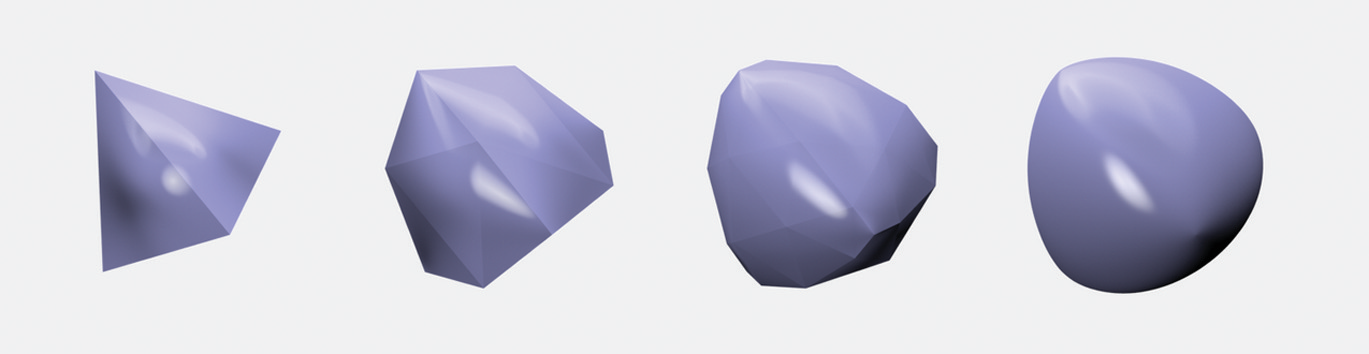
\includegraphics[width=\linewidth]{tetsubdiv.png} \caption{Image shows the tetrahedron being subdivided 0, 1, 2, 6 times} \label{fig:figure1} \end{figure*}
\begin {figure*} 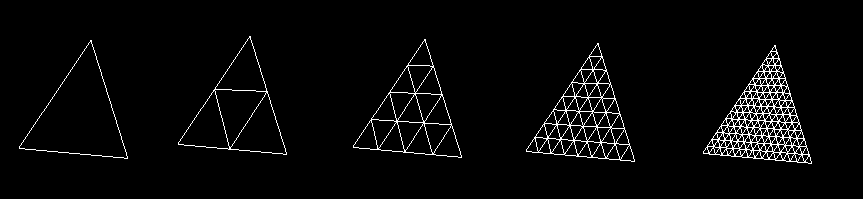
\includegraphics[width=\linewidth]{subdivision.png} \caption{shows the subdivison process on a equilateral triangle} \label{fig:figure2} \end{figure*}
this that we can have a better more refined representation of any polygon, without having to store extra information\footnote{Though, obviously we take
a memory and computation penalty for this, we can achieve a \textit{smooth limit surface}}. See in figure \ref{fig:figure1} how by subdividing a tetrahedron, 
we can approximiate a smooth surface. Usually a few iterations of this process is suffice to give a good approximation of the limit surface.

The second idea I must introduce is of normalisation, with respect to a set distance. Normally, normalisation preserves the direction of a vector, but scales it such that 
its magnitude is 1. Our normalisation is a bit different, however, because we don't end up with magnitude 1, but rather a magnitude of a set distance.

Here is a two-dimensional example of normalisation with respect to a distance:
\begin{figure*}[hbt!] 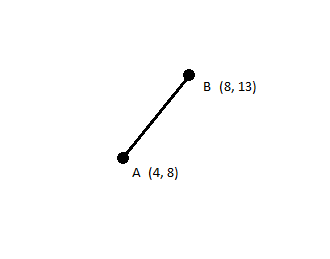
\includegraphics[width=\columnwidth]{normalA.png}\label{fig:figure2}\caption{shows two point A and B and the line between them}
\end{figure*}
\begin{figure*}[hbt!]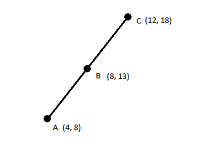
\includegraphics[width=0.5\columnwidth]{normalB.png}\label{fig:figure3}\caption[width=0.5\columnwidth]{shows the point C, which is 12 units away from A}\end{figure*}
\ref{fig:figure2} shows two points, $A$ and $B$, and the line drawn between them. Currently, the distance between $A$ and $B$ is 6 units, however if one were tasked to find
a point on the line AB that is 12 units away from $A$ (see figure \ref{fig:figure3} as point $C$).

More generally, we can say that this point $C$ will always be colinear with $A$ and $B$, but isn't nessecarily on the line segment $AB$.

Staying with the two dimension story, if we were to draw a set point of points $P$ that were all on a straight line not going through the origin,
and we were to normalise them in reference to the origin, with a certain distance $d$, we would contruct an arc of a circle with radius $d$, since all this 
exercise is, is drawing a set of points on a circle with radius $d$. It is then trivial to prove that the same would hold in three dimensions\footnote{This is a
exercise left to the reader}. 

The reason to even go through such an exercise, it to realise that we can start of a octahedron, and then subdivide it, yielding us the points on a straight line.
Then we can normalise these points to get the points on a sphere, and obviously we can also control the radius of such a sphere. To keep things simple, we use an
octahedron, because it is a comprised of 8 equilateral triangles, which are trivial to subdivide. %TODO: add some code here%

Now that we have our points that we can render, we need to somehow convert these from 3D to 2D, so that we can render them on to the screen. This is where GLM does
most of the heavy lifting, in that, we don't have to manually construct the equations to this, but can leave it up to GLM to do this for us. 
\subsubsection*{The Rendering Pipeline}
Throughout this procedure, we will be using 4D vectors ($x, y, z, w$), and 4$\times$4 matrices. The reason for this is that we can use the fourth dimension to store information
about the vector. This being
\begin{itemize}
    \item If $w = 0$, then the vector is a direction vector
    \item If $w = 1$, then the vector is a point
\end{itemize}
To begin, all of the points that describe a sphere are relative to the origin (obviously), however this origin is not nessecarily the origin
of the world (but rather relative to the origin of the model). To make it relative to the world, we can apply a \textit{model} matrix transformation.
The model matrix is consistent of:
\begin{itemize}
    \item A translation matrix -- which describes the position of the object in the world relative to the origin of the world.
    \item A rotation matrix -- which describes the orientation of the object in the world relative to the basis vectors of the world.
    \item A scaling matrix -- which describes the size of the object in the world relative to the basis vectors of the world.
\end{itemize}
After applying the model matrix, our coordinates are now in \textit{world space} (points are defined relative to the origin of the world).
Quote from Futurama:
\begin{quote}
    `The engines don't move the ship at all. The ship stays where it is and the engines move the universe around it'
\end{quote}
For example, if you want to view a mountain from a different angle, you can either move the camera or move the mountain.
Whilst not practial in real life, the latter is easier and simpler in CG than the former\@

Intially, your camera is at the origin of the world space and
you want to move your camera 3 units to the right, this would be equivalent of moving the entire world 3 units to the left instead.
Mathematically, this is equivalent of describing everything in terms of the basis vectors defined relative to the camera,
rather than in world space. This is the idea behind the view matrix; it is imperative to do this
exercise  
\end{document}